\documentclass[UTF8]{ctexart}
\usepackage{amsmath,amssymb}
\usepackage{tikz}
\usepackage{geometry}
\usetikzlibrary{calc}
\geometry{a4paper,margin=2.5cm}
\usepackage{amsmath}
\usepackage{tikz}
\usepackage{pgfplots}
\pgfplotsset{compat=1.18}







\begin{document}

\begin{titlepage}
\centering

% 背景装饰
\begin{tikzpicture}[remember picture,overlay]
\draw[blue!50, line width=6pt]
    ($(current page.north west)+(1cm,-1cm)$) --
    ($(current page.north east)+(-1cm,-1cm)$);

\draw[blue!30, line width=4pt]
    ($(current page.south west)+(1cm,1cm)$) --
    ($(current page.south east)+(-1cm,1cm)$);
\end{tikzpicture}

\vspace*{4cm}

{\Huge\bfseries Classical Problems of QM \par}

\vspace{1.5cm}

{\Large —— 量子力学经典习题 —— \par}

\vspace{3cm}

{\Large \textbf{Author: Zhao H.Q.} \par}

\vspace{0.5cm}

{\large \today \par}

\vfill

{\large \textit{Quantum Mechanics}}

\end{titlepage}

\clearpage









例题1.\\
自旋为$\frac{1}{2}$体系随时间的演化
设一粒子一开始处于$S_x=1/2$的本征态，现在加入沿Z轴的磁场$\overrightarrow{B}=B\cdot \overrightarrow{e_z}$\\
(1):请问任意t时刻粒子处于什么状态？\\
(2):请问任意t时刻处于$S_x=1/2$状态的概率是多少？$S_x=-1/2$呢？\\
(3):任意t时刻的$<\hat{S_x}>$是多少？$\hat{<S_y>}$和$\hat{<S_z>}$呢？\\

解:
粒子一开始处于$S_x=\hbar/2$状态，因此：
\[\psi(0) = |+> \]\\
要求t时刻，即:
\[\psi(t) = \hat{U}(t) \psi(0) = e^{\frac{i\hat{H}t}{\hbar}} \psi(0) \]
其中
\[\hat{H} = -\hat{\overrightarrow{\mu}} \cdot \overrightarrow{B} = -\hat{\mu_s} B = -\gamma_s \hat{S_z} B\]
其中$\gamma_s$为旋磁比

带入上式：
\[\psi(t) = e^{\frac{i \gamma_s \hat{S}_z B}{\hbar}} \cdot|+> = e^{\frac{i \gamma_s \hat{S}_z B}{\hbar}} 
\cdot (\frac{1}{\sqrt{2}} |\uparrow>) + \frac{1}{\sqrt{2}} |\downarrow> 
= e^{\frac{i \gamma_s \frac{\hbar}{2} B}{\hbar}} \cdot \frac{1}{\sqrt{2}} |\uparrow>
+e^{\frac{i \gamma_s -\frac{\hbar}{2} B}{\hbar}} \cdot \frac{1}{\sqrt{2}} |\downarrow>\]

其中：
\[
    |\uparrow> = \begin{pmatrix}
1 \\
0 
\end{pmatrix},
    |\downarrow> = \begin{pmatrix}
0 \\
1 
\end{pmatrix}
\],在Z表象

于是我们可以得到：


\[
    \psi(t) = \frac{1}{\sqrt{2}}
    \begin{pmatrix}
e^{\frac{i \gamma_s \frac{\hbar}{2} B}{\hbar}} \\
e^{\frac{i \gamma_s -\frac{\hbar}{2} B}{\hbar}} 
\end{pmatrix}
    =
    \frac{1}{\sqrt{2}} 
    \begin{pmatrix}
e^{i \omega t} \\
e^{-i \omega t} 
\end{pmatrix}
\]\\

(2):t时刻处于$S_x=\frac{\hbar}{2}$和$-\frac{\hbar}{2}$的概率
\[  
    P_{\frac{\hbar}{2}} = | <+|\psi(t)> |^2
    = [\frac{1}{\sqrt{2}}(1,1)\cdot \frac{1}{\sqrt{2}}
    \begin{pmatrix}
e^{i \omega t} \\
e^{-i \omega t} 
\end{pmatrix}]^2
    =cos^2(\omega t)
\]

注：其中用了欧拉公式：$e^{i\omega}=cos\omega + isin\omega$

与上式同理可求得
\[
    P_{\frac{\hbar}{2}}=sin^2(\omega t)
\]

(3):t时刻$S_z,S_x,S_y$的平均值：

\[
 <\hat{S}_x> = < \psi(t)| \hat{S}_x |\psi(t) >
 = \frac{1}{\sqrt{2}}(e^{i \omega t},e^{-i \omega t}) \cdot \frac{\hbar}{2} 
 \begin{pmatrix}
  0&1 \\
  1&0
\end{pmatrix}
 \frac{1}{\sqrt{2}}
  \begin{pmatrix}
   e^{i \omega t}\\
  e^{-i \omega t}
\end{pmatrix}
    = \frac{\hbar}{2} cos(2\omega t)
\]\\
同理可得：

\[
    <\hat{S}_y> = \frac{\hbar}{2} sin(2\omega t)
\]
\[<\hat{S}_z> = 0\]

相当于粒子在XoY平面上做Lammor进动\\






例题2.\\
一个质量为$\mu$的粒子在一维势场中：

\[
V(x)=
\begin{cases}
0, & |x| > a \\
- V_0, & |x| < a
\end{cases}
\]

运动，其中$V_0>0$，求存在且仅存在一个解的条件

\begin{figure}[htbp]
    \centering
    \begin{tikzpicture}
            % 坐标轴
    \draw[->] (-4.5,0) -- (4.8,0) node[right] {$x$};
    \draw[->] (0,-3.5) -- (0,1.5) node[above] {$V(x)$};

    % 势井（井内为 -V0）
    \draw[thick]
        (-4,0) -- (-1.5,0)
        -- (-1.5,-2.5) -- (1.5,-2.5)
        -- (1.5,0) -- (4,0);

    % 标注 0 势能
    \node[left] at (0,0) {$0$};

    % 标注 -V0
    \draw[dashed] (-4.2,-2.5) -- (4.2,-2.5);
    \node[left] at (0,-2.5) {$-V_0$};

    % 边界
    \draw[dashed] (-1.5,0) -- (-1.5,-2.5);
    \draw[dashed] (1.5,0) -- (1.5,-2.5);
    \node[above] at (-1.5,0) {$-a$};
    \node[above] at (1.5,0) {$a$};

    % 区域标注
    \node at (0,-1.2) {势井区域};
    \end{tikzpicture}
    \caption{有限深势井示意图}
\end{figure}

将上式带入定态薛定谔方程：\\
\[
V(x)=
\begin{cases}
-\frac{\hbar^2}{2m}\frac{d^2}{dx^2}\psi(x) =E \psi(x) , & |x| > a \\
-\frac{\hbar^2}{2m}\frac{d^2}{dx^2}\psi(x) =(E+V_0)\psi(x)& |x| < a
\end{cases}
\]

其解为：
\[
V(x)=
\begin{cases}
\psi_1(x)=C_1e^{\sqrt{\frac{-2mE}{\hbar^2}}x}  + C_2e^{-\sqrt{\frac{-2mE}{\hbar^2}}x}  , & |x| > a \\
\psi_2(x)=C_3e^{\sqrt{\frac{-2m(E+V_0)}{\hbar^2}}x}  + C_4e^{-\sqrt{\frac{-2m(E+V_0)}{\hbar^2}}x} & |x| < a
\end{cases}
\]

\[
    \rightarrow
    \begin{cases}
\psi_1(x)=C_1e^{\alpha x}  + C_2e^{-\alpha x}  , & |x| > a \\
\psi_2(x)=C_3e^{i \beta x}  + C_4e^{-i\beta x} & |x| < a
\end{cases}
\]

\[
    \rightarrow\\
    \psi_2(x) = C_5cos(\beta x) + C_6sin(\beta x) , |x|\le a
\]\\

这里我们先不带入边界条件求解，我们注意到势场是偶函数，则$\psi(x)$具有确定的宇称(奇偶不能确定)，下面我们分情况讨论： \\
(1):偶宇称：\\
有边界条件：$\psi(x)$在边界处连续，一阶导数在边界处(非奇异点)也连续：\\
\[
    \begin{cases}
        C_1 = C_2 =A \\
        A e^{\alpha x},x>a\\
        A e^{\alpha x},x<-a\\
        C_5 = B\\
        B cos(\beta x),|x|\le a
    \end{cases}
\]
联立求解我们可以得到：
\[
    \xi tan(\xi) = \eta
\]
其中：
\[
    \begin{aligned}
        \xi = \beta a\\
        \eta = \alpha a
    \end{aligned}
\]
\\
下面我们来考虑奇宇称的情况：
(2):奇宇称：\\
有边界条件：$\psi(x)$在边界处连续，一阶导数在边界处(非奇异点)也连续：\\
\[
    \begin{cases}
        C_1 = -C_2 =A' \\
        A' e^{\alpha x},x>a\\
        -A' e^{\alpha x},x<-a\\
        C_6 = B'\\
        B' sin(\beta x),|x|\le a
    \end{cases}
\]
联立求解我们可以得到：
\[
    \xi cot(\xi) = -\eta
\]
这里根据$\xi$和$\eta$的定义，有：
\[
    \xi^2 + \eta^2 = \frac{2m a^2 V_0}{\hbar^2} = Q^2
\]
也就是说$\xi$和$\eta$
应该同时满足超越方程和圆方程：

现在的结果已经比较清晰了，我们只要找到圆和超越方程对应图形的交点即可知道有几个束缚态，下面是示意图：


\begin{figure}[htbp]
    \centering
    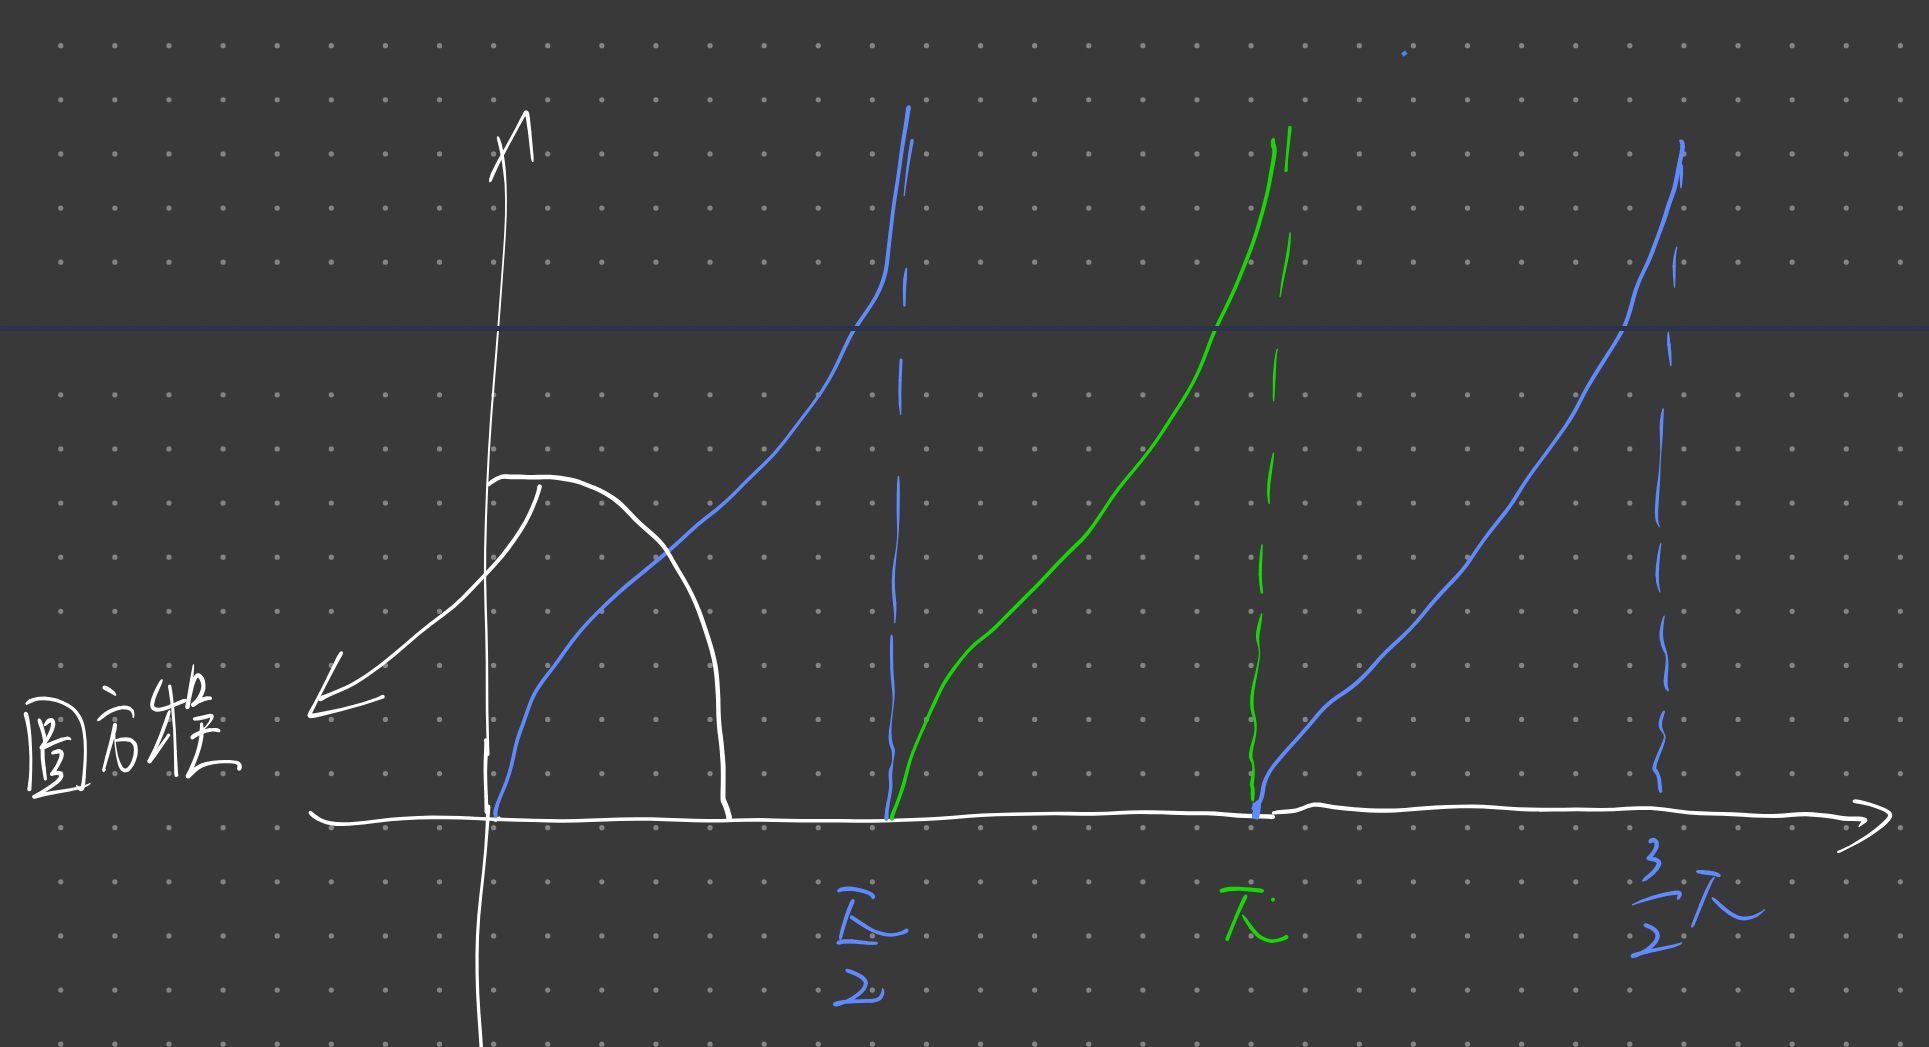
\includegraphics[width=0.6\textwidth]{figs/1.png}
    \caption{示意图(蓝色为tan，绿色为cot)}
    \label{fig:example}
\end{figure}

\newpage
结果，当：
\[
    \sqrt{\frac{2ma^2 V_0}{\hbar^2}} < \frac{\pi}{2}
\]
时，仅有一个束缚态\\


例题3.\\
已知电子某一时刻的波函数为$\Psi(r,t)=\Psi_1(r,t)\chi_+(S_z)+\Psi_2(r,t)\chi_-(S_z)$,其中$\chi_+(S_z)$与$\chi_-(S_z)$
分别是电子自旋沿正z轴与负z轴的归一化波函数.试写出电子自旋沿正z轴且在薄壳(r,r+dr)内出现的概率$P_1$;电子自旋沿负z轴且在$(\theta,\phi)$方向$d\Omega=sin\theta d\theta d\phi$
立体角内出现的概率$P_2$;电子自旋沿正z轴的概率$P_3$\\

在$\hat{S}_z$表象下:
\[
    \chi_+=
    \begin{bmatrix}
        1\\
        0
    \end{bmatrix}
     \chi_-=
    \begin{bmatrix}
        0\\
        1
    \end{bmatrix}
\]

考虑自旋的波函数,可以将其写成旋量形式:
\[
    \psi(r,t)=
    \begin{bmatrix}
        \psi_1(r,t)\\
        \psi_2(r,t)
    \end{bmatrix}
\]
其中$\psi_1(r,t)$代表自旋向上部分的空间波函数,然后将其归一化,使得:\\

\[
    \int_{-\infty}^{\infty} \tilde{\psi}(r,t)^*\cdot \tilde{\psi}(r,t) = 1
\]
于是我们可以得到：

\[
    \tilde{\psi}(r,t) = N \cdot 
    \begin{bmatrix}
        \psi_1(r,t)\\
        \psi_2(r,t)
    \end{bmatrix}
\]

其中:
\[
    N = \frac{1}{\sqrt{  \int_{-\infty}^{\infty}|\psi_1|^2 d\tau + \int_{-\infty}^{\infty}|\psi_2|^2 d\tau}}
\]
因此,归一化波函数的模方表示概率,则电子自旋沿Z轴向上的概率为:
\[
    P_{\uparrow} =  \int_{-\infty}^{\infty}|N \psi_1|^2 d\tau = \frac{ \int_{-\infty}^{\infty}|\psi_1|^2 d\tau}{ \int_{-\infty}^{\infty}|\psi_1|^2 d\tau + \int_{-\infty}^{\infty}|\psi_2|^2 d\tau }
\]

\[
    P_{\downarrow} =  \int_{-\infty}^{\infty}|N \psi_2|^2 d\tau = \frac{ \int_{-\infty}^{\infty}|\psi_2|^2 d\tau}{ \int_{-\infty}^{\infty}|\psi_1|^2 d\tau + \int_{-\infty}^{\infty}|\psi_2|^2 d\tau }
\]
\\
下面我们求在(r,r+dr)范围内,沿着Z轴向上的概率.\\
\\
注意这里有一个易错点;并不能用概率公式:$P(A \cap B)=P(A)\cdot P(B)$,因为此时"沿着Z轴向上"和"在某处找到粒子"这两件事并不独立,相当于知道"沿着Z轴向上"时
,已经做了一次挑选(或测量),因此这里我们的波函数应该落入归一化后的$\psi_1$\\

(1):
\[
    P_1 = P_{\uparrow} \cdot P(r \to r+dr)
    =P_{\uparrow} \cdot \int_{\Omega} \frac{|\psi_1|^2 d\tau}{  \int_{-\infty}^{\infty}|\psi_1|^2 d\tau }
    =P_{\uparrow} \cdot r^2dr \int_{0}^{\pi}\int_{2\pi}^{0}\frac{|\psi_1|^2 sin\theta d\theta d\phi}{\int_{-\infty}^{\infty}|\psi_1|^2 d\tau}
\]

(2):
\[
    P_1 = P_{\downarrow} \cdot P(\theta,\phi)
    =P_{\downarrow} \cdot \int_{-\infty}^{\infty} \frac{|\psi_2|^2 d\tau}{  \int_{-\infty}^{\infty}|\psi_2|^2 d\tau }
    =P_{\downarrow} \cdot sin\theta d\theta d\psi \int_{-\infty}^{\infty}\frac{|\psi_1|^2 r^2dr}{\int_{-\infty}^{\infty}|\psi_2|^2 d\tau}
\]

(3):
\[
    P_3=P_{\uparrow}
\]
\\

例题4:
\\
三维球势阱中，某粒子在球壳中运动：
\[
    V(r) = 
    \begin{cases}
        0 & 0<r<a\\
        \infty & r>a
    \end{cases}
\]
求l=0时的本征值与本征函数：

考虑到势场具有球对称性，可以取中心立场类似的CSCO$(\hat{L^2},\hat{L_z},\hat{H})$则可设本征函数：
\[
    \psi(r,\theta,\phi) = R(r)\cdot Y_l^m(\theta,\phi)
\]

TISE:
\[
    [-\frac{\hbar^2}{2m}\frac{\partial^2}{\partial r^2}u(r) + \frac{l(l+1)\hbar^2}{2mr^2}u(r)+V(r)U(r)] = E u(r)
\]
由于球壳外$V(r)=\infty$,则$\psi(r,\theta,\phi)|_{r>a}=0$,我们只用考虑球壳内部的波函数(内部l=0)：

\[
    -\frac{\hbar^2}{2m} u(r) = E u(r)
\]
注意到这个方程与一维无限深方势阱的方程一致，边界条件：
\[
    \begin{cases}
    u(0)=0\\
    u(a)=0
    \end{cases}
\]

边界条件也与一维无限深方势阱一致，则解与一维无限深方势阱的解形式一模一样，只需将x替换为r即可：
\[
    u(r) = \sqrt{\frac{2}{a}} sin\frac{n \pi r}{a} , E_n\frac{n^2 \pi^2 \hbar^2}{2ma^2}
\]
\[
    R(r) = \frac{1}{r} \sqrt{\frac{2}{a}} sin\frac{n \pi r}{a}
\]
得到最终的总体空间波函数：
\[
    \psi_{n,m,l}(r,\theta ,\phi) = \frac{1}{r} \sqrt{\frac{2}{a}} sin\frac{n \pi r}{a} \cdot Y_l^m(\theta,\phi)|^{m=0}_{l=0}= \frac{1}{r \sqrt{4\pi}} \sqrt{\frac{2}{a}} sin\frac{n \pi r}{a} 
\]\\

例题5:\\
求基态氢原子电子最可能出现的半径。\\ \\
注：这里对于氢原子空间总体波函数的求解不做赘述，详情请见我的"量子力学随笔.pdf"\\

氢原子电子空间波函数：
\[
    \psi_{n,l,m}(r,\theta,\phi) = \alpha_0\sum_{i=0}^{n-l-1}\frac{2^i}{i!}\frac{r^{l+1}}{a_0 n} e^{-\frac{r}{a_0 n}} Y_l^m(\theta,\phi)
\]
经过归一化后:
\[
    \psi_{100} = \frac{1}{\sqrt{\pi a_0^3}}e^{-\frac{r}{a_0}}
\]

这里注意到基态波函数与角向无关，现考虑氢原子径向概率密度:
\[
    \rho(r) = |\psi_{100}|^2
\]
在某球壳$r\rightarrow r+dr$的概率：

\[
    P_{r\rightarrow r+dr}=4\pi r^2\cdot \frac{1}{\pi a_0^3}e^{-\frac{2r}{a_0}} dr
\]
在概率表达式中的dr项只是个测度，除去dr的项也可以表征概率大小，令$P=P_{r\rightarrow r+dr}/dr$
\[
    \frac{dP}{dr} = 0
    \rightarrow \frac{4}{a_0^3}[e^{-\frac{2r}{a_0}}\cdot 2r + (-\frac{2}{a_0})e^{-\frac{2r}{a_0}}r]=0
\]
解得：$r=a_0$\\
因此$a_0$就是基态氢原子中电子最可能出现的半径，称为(第一)Bhor半径



\end{document}